\begin{figure}
  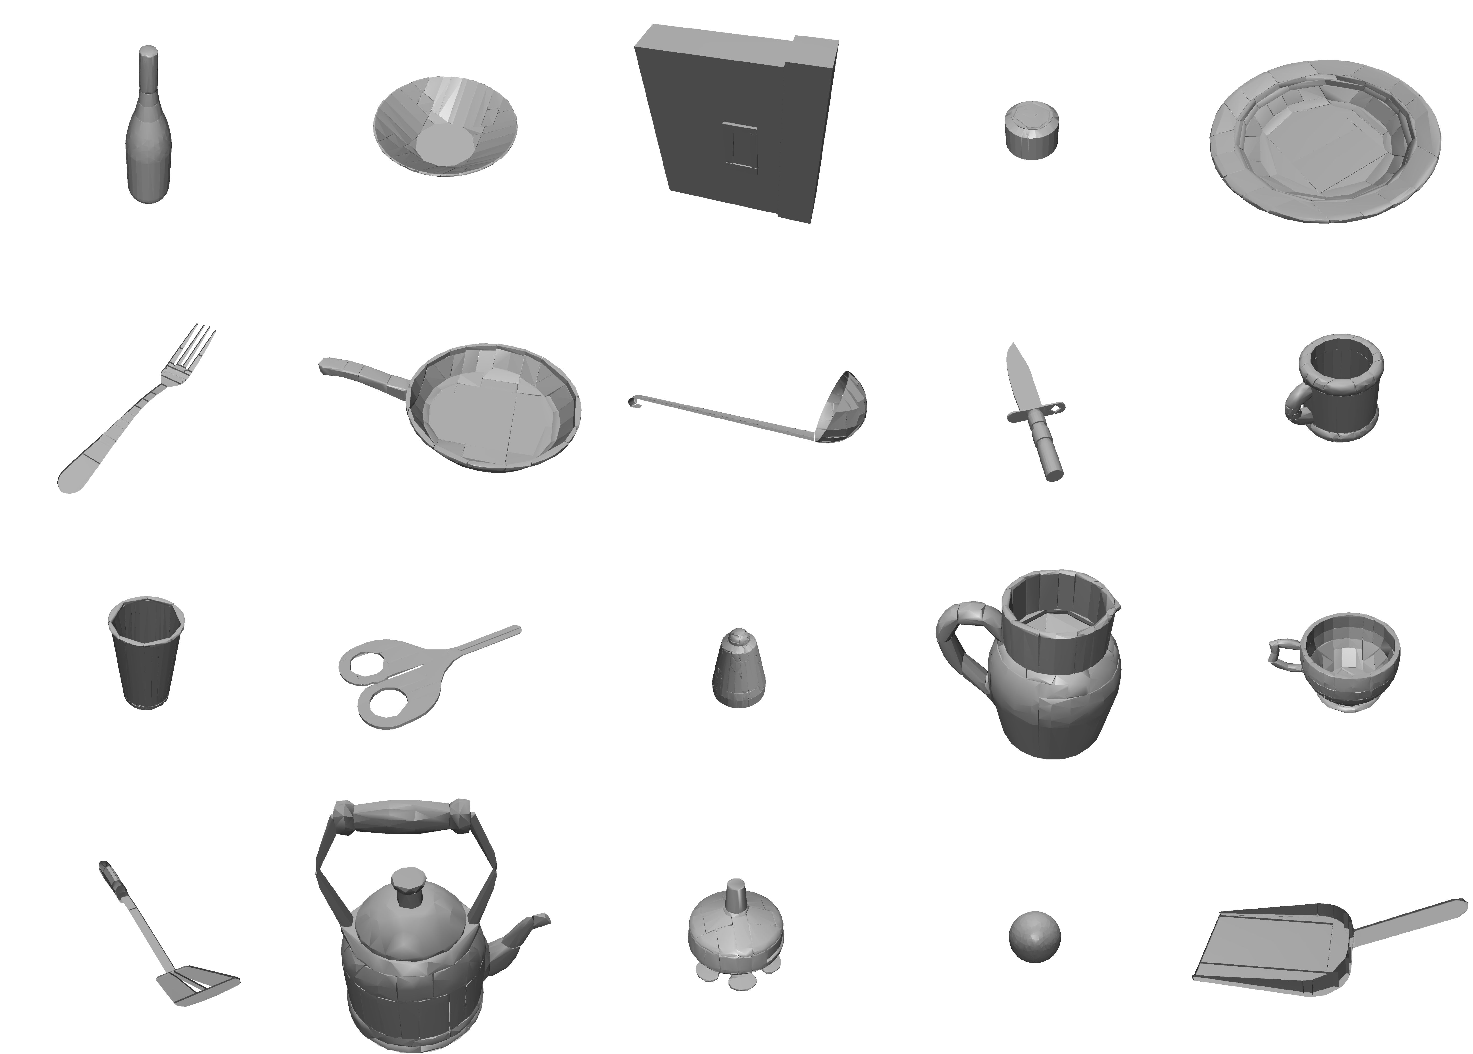
\includegraphics[width=\linewidth]{images/allObjects.pdf}
  \caption{Sample objects from all classes in the 3D model dataset.}
  \label{fig:allObjects}
\end{figure}

In order to test our grasp success prediction network, we have used 49 scenes of 40 previously unseen real objects. The highest-ranked grasp based on the predicted success probability of the network is performed on each scene. Out of all 40 objects used to test the method, 35 belonged to the object classes we have in our simulation dataset, while the remaining 5 belong to categories that do not exist in the simulation set. 

Our shape collection dataset consists of 294 objects from 20 classes. The number of objects in each class varies between 25 (bottles) and 1 (dustpan). 250 objects from all classes have been used for training the network, while the remaining 44 has been used for validation in simulation. The objects included in simulation are graspable everyday objects having different characteristics. Examples are kitchen objects such as bowls, plates, mugs and teacups, solid objects such as boxes and balls, kitchen utensils such as spatulas, spoons. Long/thin objects such as spatula, fork, spoon, knife classes are placed on a heavy cup vertically in order to make them graspable without touching the table. 

Training parameters for network. Training of example grasps for learning from demonstration. Creation of real test data set. Paired comparisons methodology with vanilla LFD algorithm (pose + object + camera view).

The actual grasping tests have been performed on the real robot. 